% Pan-cancer multi-agent tumour segmentation and reasoning pipeline (Fig. pipeline). Standalone TikZ; compile with pdflatex.
\documentclass[tikz,border=4pt]{standalone}
\usepackage[scaled=0.92]{helvet}
\renewcommand{\familydefault}{\sfdefault}
\usepackage{sfmath}
\usepackage{amsmath,amssymb}
\usetikzlibrary{arrows.meta,positioning,calc,fit,backgrounds,shapes.misc}

% palette (muted; groups distinguished by hue and by labels)
\definecolor{ink}{HTML}{1F2933}
\definecolor{mute}{HTML}{5B6670}
\definecolor{inF}{HTML}{F1F3F5}\definecolor{inD}{HTML}{5B6670}
\definecolor{kbF}{HTML}{FCF1D8}\definecolor{kbD}{HTML}{A8670A}
\definecolor{agF}{HTML}{E3ECFA}\definecolor{agD}{HTML}{2B5BAA}
\definecolor{rsF}{HTML}{DFF3EF}\definecolor{rsD}{HTML}{17766A}
\definecolor{imF}{HTML}{C9EBE4}
\definecolor{ouF}{HTML}{ECE6F8}\definecolor{ouD}{HTML}{5E3EA8}
\definecolor{rjF}{HTML}{F9E0DE}\definecolor{rjD}{HTML}{A23B32}
\definecolor{rvF}{HTML}{E2F2E0}\definecolor{rvD}{HTML}{3D7A34}
\definecolor{rcF}{HTML}{DDEEF8}\definecolor{rcD}{HTML}{25679A}
\definecolor{tuF}{HTML}{F6D9D5}\definecolor{orF}{HTML}{DCEFEA}

\tikzset{
  box/.style={draw=#1, line width=0.7pt, rounded corners=3pt, align=left, inner sep=4pt, text=ink},
  ttl/.style={font=\bfseries\footnotesize, text=ink, anchor=north west, align=left},
  txt/.style={font=\scriptsize, text=ink, anchor=north west, align=left},
  arr/.style={-{Stealth[length=5pt,width=4pt]}, line width=0.8pt, color=ink!80},
  dar/.style={arr, dashed},
  lab/.style={font=\tiny, text=mute, fill=white, inner sep=1pt, align=center},
  chip/.style={draw=#1, fill=#1!12, rounded corners=6pt, font=\scriptsize\bfseries, text=#1, inner sep=2.5pt, minimum width=1.25cm},
  slot/.style={draw=agD!70, fill=white, rounded corners=2pt, line width=0.5pt, text width=4.05cm, align=left, inner sep=3pt},
  hdr/.style={font=\bfseries\small, text=ink, anchor=south west},
  gnode/.style={draw=#1, line width=0.6pt, rounded corners=2pt, font=\tiny, inner sep=2pt, align=center, text=ink},
}

\begin{document}
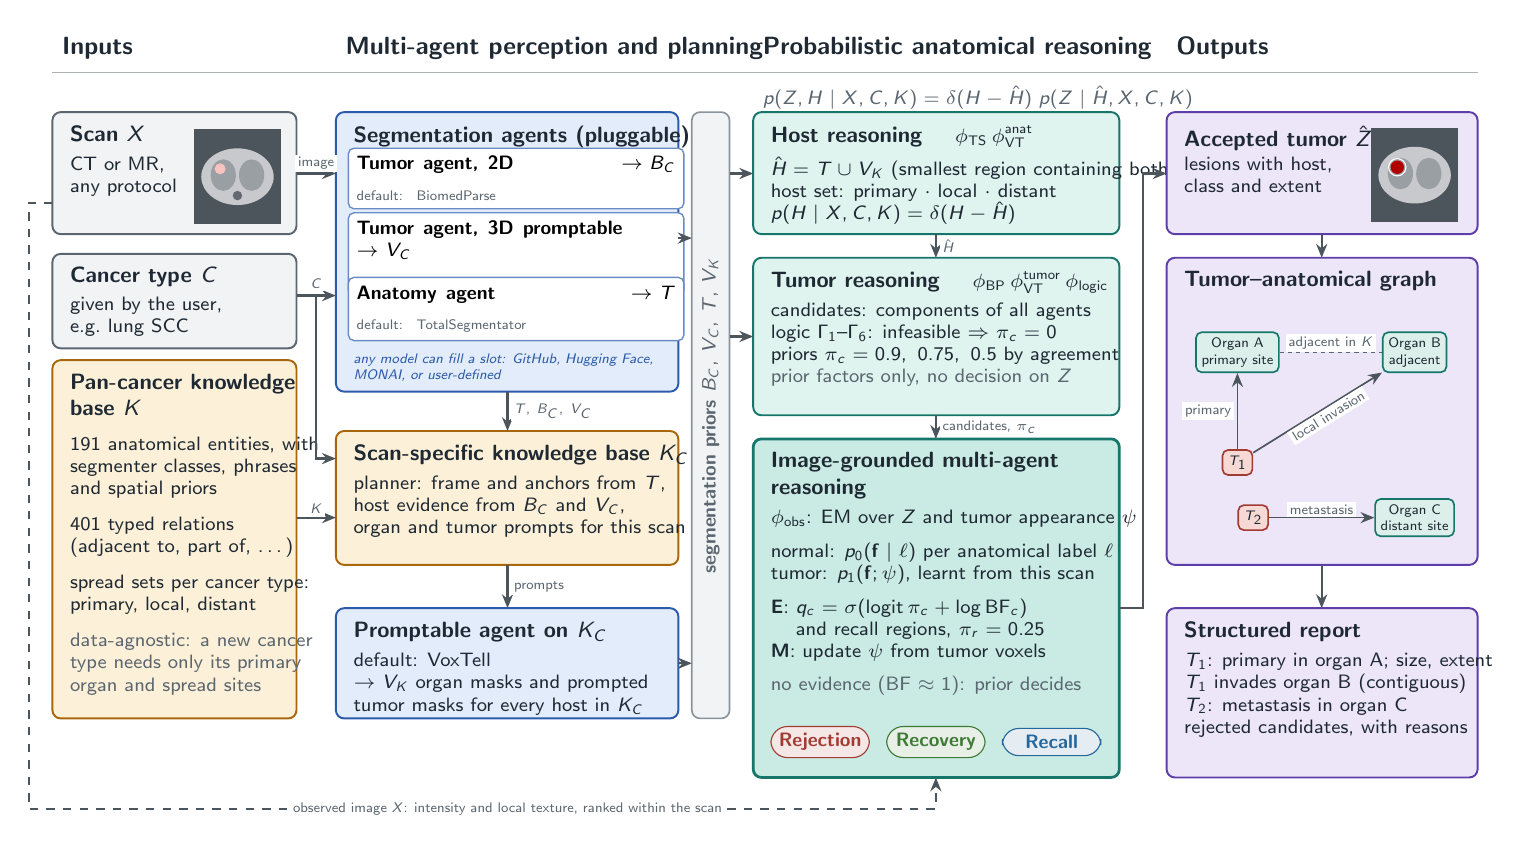
\begin{tikzpicture}[x=1cm,y=1cm]

% ------------------------------------------------------------------ column headers
\node[hdr] at (0,10.15) {Inputs};
\node[hdr] at (3.6,10.15) {Multi-agent perception and planning};
\node[hdr] at (8.9,10.15) {Probabilistic anatomical reasoning};
\node[hdr] at (14.15,10.15) {Outputs};
\draw[mute!50, line width=0.4pt] (0,10.1) -- (18.1,10.1);
\node[font=\scriptsize, text=mute, anchor=north west] at (8.9,10.05)
  {$p(Z,H\mid X,C,K)=\delta(H-\hat H)\;p(Z\mid \hat H,X,C,K)$};

% ------------------------------------------------------------------ column 1: inputs
\draw[box=inD, fill=inF] (0,8.05) rectangle (3.1,9.6);
\node[ttl] at (0.1,9.55) {Scan $X$};
\node[txt] at (0.1,9.15) {CT or MR,\\any protocol};
% stylised axial slice
\begin{scope}[shift={(2.35,8.78)}]
  \fill[ink!80] (-0.55,-0.6) rectangle (0.55,0.6);
  \fill[ink!25] (0,0) ellipse (0.46 and 0.36);
  \fill[ink!45] (-0.18,0.02) ellipse (0.16 and 0.2);
  \fill[ink!45] (0.18,0.02) ellipse (0.16 and 0.2);
  \fill[tuF!90!red] (-0.22,0.1) circle (0.07);
  \fill[ink!70] (0,-0.24) circle (0.06);
\end{scope}

\draw[box=inD, fill=inF] (0,6.6) rectangle (3.1,7.8);
\node[ttl] at (0.1,7.75) {Cancer type $C$};
\node[txt] at (0.1,7.38) {given by the user,\\e.g.\ lung SCC};

\draw[box=kbD, fill=kbF] (0,1.9) rectangle (3.1,6.45);
\node[ttl] at (0.1,6.4) {Pan-cancer knowledge\\base $K$};
\node[txt] at (0.1,5.6) {%
  191 anatomical entities, with\\segmenter classes, phrases\\and spatial priors\\[5pt]
  401 typed relations\\(adjacent to, part of, \ldots)\\[5pt]
  spread sets per cancer type:\\primary, local, distant\\[5pt]
  {\color{mute}data-agnostic: a new cancer}\\{\color{mute}type needs only its primary}\\{\color{mute}organ and spread sites}};

% ------------------------------------------------------------------ column 2: agents, planner, prompted agent
\draw[box=agD, fill=agF] (3.6,6.05) rectangle (7.95,9.6);
\node[ttl] at (3.7,9.55) {Segmentation agents (pluggable)};
\node[slot, anchor=north west] (s1) at (3.75,9.15) {\scriptsize\textbf{Tumor agent, 2D}\hfill $\to B_C$\\[-1pt]\tiny\color{mute} default: BiomedParse};
\node[slot, anchor=north west] (s2) at (3.75,8.33) {\scriptsize\textbf{Tumor agent, 3D promptable}\hfill $\to V_C$\\[-1pt]\tiny\color{mute} default: VoxTell};
\node[slot, anchor=north west] (s3) at (3.75,7.51) {\scriptsize\textbf{Anatomy agent}\hfill $\to T$\\[-1pt]\tiny\color{mute} default: TotalSegmentator};
\node[font=\tiny\itshape, text=agD, anchor=north west, align=left] at (3.7,6.66)
  {any model can fill a slot: GitHub, Hugging Face,\\MONAI, or user-defined};

\draw[box=kbD, fill=kbF] (3.6,3.85) rectangle (7.95,5.55);
\node[ttl] at (3.7,5.5) {Scan-specific knowledge base $K_C$};
\node[txt] at (3.7,5.1) {%
  planner: frame and anchors from $T$,\\host evidence from $B_C$ and $V_C$,\\organ and tumor prompts for this scan};

\draw[box=agD, fill=agF] (3.6,1.9) rectangle (7.95,3.3);
\node[ttl] at (3.7,3.25) {Promptable agent on $K_C$};
\node[txt] at (3.7,2.85) {%
  default: VoxTell\\
  $\to V_K$ organ masks and prompted\\tumor masks for every host in $K_C$};

% ------------------------------------------------------------------ prior bus
\draw[draw=mute!70, fill=inF, rounded corners=3pt, line width=0.6pt] (8.12,1.9) rectangle (8.6,9.6);
\node[rotate=90, font=\scriptsize\bfseries, text=mute] at (8.36,5.75) {segmentation priors $B_C,\,V_C,\,T,\,V_K$};

% ------------------------------------------------------------------ column 3: reasoning
\draw[box=rsD, fill=rsF] (8.9,8.05) rectangle (13.55,9.6);
\node[ttl] at (9.0,9.55) {Host reasoning \quad\normalfont\scriptsize$\phi_{\mathrm{TS}}\,\phi^{\mathrm{anat}}_{\mathrm{VT}}$};
\node[txt] at (9.0,9.15) {%
  $\hat H=T\cup V_K$ (smallest region containing both)\\
  host set: primary $\cdot$ local $\cdot$ distant\\
  $p(H\mid X,C,K)=\delta(H-\hat H)$};

\draw[box=rsD, fill=rsF] (8.9,5.75) rectangle (13.55,7.75);
\node[ttl] at (9.0,7.7) {Tumor reasoning \quad\normalfont\scriptsize$\phi_{\mathrm{BP}}\,\phi^{\mathrm{tumor}}_{\mathrm{VT}}\,\phi_{\mathrm{logic}}$};
\node[txt] at (9.0,7.3) {%
  candidates: components of all agents\\
  logic $\Gamma_1$--$\Gamma_6$: infeasible $\Rightarrow \pi_c=0$\\
  priors $\pi_c=0.9,\ 0.75,\ 0.5$ by agreement\\
  {\color{mute}prior factors only, no decision on $Z$}};

\draw[box=rsD, fill=imF, line width=1pt] (8.9,1.15) rectangle (13.55,5.45);
\node[ttl] at (9.0,5.4) {Image-grounded multi-agent\\reasoning\\[1pt]\normalfont\scriptsize$\phi_{\mathrm{obs}}$: EM over $Z$ and tumor appearance $\psi$};
\node[txt] at (9.0,4.25) {%
  normal: $p_0(\mathbf f\mid\ell)$ per anatomical label $\ell$\\
  tumor: $p_1(\mathbf f;\psi)$, learnt from this scan\\[4pt]
  \textbf{E}: $q_c=\sigma(\operatorname{logit}\pi_c+\log \mathrm{BF}_c)$\\
  \phantom{\textbf{E}: }and recall regions, $\pi_r=0.25$\\
  \textbf{M}: update $\psi$ from tumor voxels\\[4pt]
  {\color{mute}no evidence ($\mathrm{BF}\approx1$): prior decides}};
\node[chip=rjD] (c1) at (9.75,1.6) {Rejection};
\node[chip=rvD] (c2) at (11.22,1.6) {Recovery};
\node[chip=rcD] (c3) at (12.69,1.6) {Recall};

% ------------------------------------------------------------------ column 4: outputs
\draw[box=ouD, fill=ouF] (14.15,8.05) rectangle (18.1,9.6);
\node[ttl] at (14.25,9.55) {Accepted tumor $\hat Z$};
\node[txt] at (14.25,9.15) {lesions with host,\\class and extent};
\begin{scope}[shift={(17.3,8.8)}]
  \fill[ink!80] (-0.55,-0.6) rectangle (0.55,0.6);
  \fill[ink!25] (0,0) ellipse (0.46 and 0.36);
  \fill[ink!45] (-0.18,0.02) ellipse (0.16 and 0.2);
  \fill[ink!45] (0.18,0.02) ellipse (0.16 and 0.2);
  \fill[red!70!black] (-0.22,0.1) circle (0.085);
  \draw[white, line width=0.4pt] (-0.22,0.1) circle (0.11);
\end{scope}

\draw[box=ouD, fill=ouF] (14.15,3.85) rectangle (18.1,7.75);
\node[ttl] at (14.25,7.7) {Tumor--anatomical graph};
\node[gnode=rsD, fill=orF] (oA) at (15.05,6.55) {Organ A\\primary site};
\node[gnode=rsD, fill=orF] (oB) at (17.3,6.55) {Organ B\\adjacent};
\node[gnode=rsD, fill=orF] (oC) at (17.3,4.45) {Organ C\\distant site};
\node[gnode=rjD, fill=tuF] (t1) at (15.05,5.15) {$T_1$};
\node[gnode=rjD, fill=tuF] (t2) at (15.25,4.45) {$T_2$};
\draw[arr, line width=0.6pt] (t1) -- node[lab, left, xshift=-1pt] {primary} (oA);
\draw[arr, line width=0.6pt] (t1) -- node[lab, pos=0.55, below, sloped] {local invasion} (oB);
\draw[arr, line width=0.6pt] (t2) -- node[lab, above] {metastasis} (oC);
\draw[mute, line width=0.5pt, dash pattern=on 1.5pt off 1.5pt] (oA) -- node[lab, above] {adjacent in $K$} (oB);

\draw[box=ouD, fill=ouF] (14.15,1.15) rectangle (18.1,3.3);
\node[ttl] at (14.25,3.25) {Structured report};
\node[txt] at (14.25,2.85) {%
  $T_1$: primary in organ A; size, extent\\
  $T_1$ invades organ B (contiguous)\\
  $T_2$: metastasis in organ C\\
  rejected candidates, with reasons};

% ------------------------------------------------------------------ arrows
% inputs -> agents
\draw[arr] (3.1,8.82) -- node[lab, above] {image} (3.6,8.82);
\coordinate (cj) at (3.35,7.27);
\draw[arr] (3.1,7.27) -- (3.6,7.27);
\node[lab, above] at (3.35,7.32) {\,$C$\,};
% C and K -> planner
\draw[arr] (cj) -- (3.35,5.2) -- (3.6,5.2);
\draw[arr] (3.1,4.45) -- node[lab, above] {$K$} (3.6,4.45);
% agents -> planner (evidence), planner -> prompted agent
\draw[arr] (5.78,6.05) -- node[lab, right, xshift=1pt] {$T,\,B_C,\,V_C$} (5.78,5.55);
\draw[arr] (5.78,3.85) -- node[lab, right, xshift=1pt] {prompts} (5.78,3.3);
% agents and prompted agent -> prior bus
\draw[arr] (7.95,8.0) -- (8.12,8.0);
\draw[arr] (7.95,2.6) -- (8.12,2.6);
% prior bus -> host, tumour
\draw[arr] (8.6,8.82) -- (8.9,8.82);
\draw[arr] (8.6,6.75) -- (8.9,6.75);
% host -> tumour -> image-grounded
\draw[arr] (11.22,8.05) -- node[lab, right, xshift=1pt] {$\hat H$} (11.22,7.75);
\draw[arr] (11.22,5.75) -- node[lab, right, xshift=1pt] {candidates, $\pi_c$} (11.22,5.45);
% image X -> image-grounded (along the bottom)
\draw[dar] (0,8.45) -- (-0.3,8.45) -- (-0.3,0.75) -- (11.22,0.75) -- (11.22,1.15);
\node[lab] at (5.78,0.75) {observed image $X$: intensity and local texture, ranked within the scan};
% image-grounded -> accepted -> graph -> report
\draw[arr] (13.55,3.3) -- (13.85,3.3) -- (13.85,8.82) -- (14.15,8.82);
\draw[arr] (16.12,8.05) -- (16.12,7.75);
\draw[arr] (16.12,3.85) -- (16.12,3.3);

\end{tikzpicture}
\end{document}
